\documentclass[a4paper,12pt]{report}

\usepackage{cmap}
\usepackage[T2A]{fontenc}
\usepackage[utf8]{inputenc}
\usepackage[english,russian]{babel}
\usepackage{listings}
\usepackage{amsmath}
\usepackage{float}
\usepackage{csquotes}

\usepackage{xcolor}
\usepackage{hyperref}

\usepackage{graphicx}
\graphicspath{ {./images/} }

\definecolor{dkgreen}{rgb}{0,0.6,0}
\definecolor{gray}{rgb}{0.5,0.5,0.5}
\definecolor{mauve}{rgb}{0.58,0,0.82}

\lstset{
    language=Python,                 % выбор языка для подсветки (здесь это С)
    basicstyle=\small\sffamily, % размер и начертание шрифта для подсветки кода
    numbers=left,               % где поставить нумерацию строк (слева\справа)
    numberstyle=\tiny,           % размер шрифта для номеров строк
    stepnumber=1,                   % размер шага между двумя номерами строк
    numbersep=5pt,                % как далеко отстоят номера строк от подсвечиваемого кода
    aboveskip=3mm,
    belowskip=3mm,
    showstringspaces=false,
    columns=flexible,
    captionpos=b, 
    basicstyle={\small\ttfamily},
    numbers=left,
    numberstyle=\tiny\color{gray},
    keywordstyle=\color{blue},
    commentstyle=\color{mauve},
    stringstyle=\color{dkgreen},
    breaklines=true,
    breakatwhitespace=true,
    tabsize=3
}

\title{Лабораторная работа №1\\Звуки и сигналы}
\author{Кобыжев Александр}
\date{\today}

\begin{document}

\maketitle
\tableofcontents
\listoffigures
\lstlistoflistings

\maketitle

\chapter{Упражнение 1.1}

В данном упражнении нас просят открыть \texttt{chap01.ipynb}, прочитать пояснения, а также запустить примеры. Под самый конец блокнота стало жалко скрипку, точнее что с ней сделали виджеты IPython.

\chapter{Упражнение 1.2}
\section{Скачивание звука и работа с ним}

С предложенного нам сайта скачан звук работы какого-то механизма. Ссылка на соответствующий звук:

\href{https://freesound.org/people/felix.blume/sounds/414062/}{https://freesound.org/people/felix.blume/sounds/414062/}.

Далее звук был загружен, прослушан, и получена его визуализация.

\begin{lstlisting}[caption=Загрузка и прослушивание звука]
wave = thinkdsp.read_wave('sounds/414062__felix-blume__machine-gears.wav')
wave.normalize()
wave.make_audio()
\end{lstlisting}

\begin{lstlisting}[caption=Визуализация звука]
wave.plot()
\end{lstlisting}

\begin{figure}[H]
        \centering
        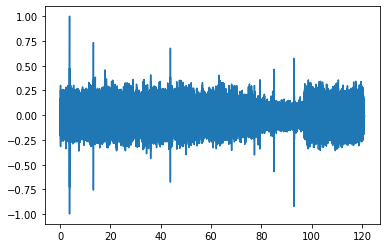
\includegraphics[width=0.75\textwidth]{lab1_fig2_1.png}
        \caption{Исходный звук}
        \label{fig:lab1_fig2_1}
\end{figure}
    
Далее возьмём полусекундный сегмент звука.

\begin{lstlisting}[caption=Изменение и прослушивание звука]
segment = wave.segment(start=25, duration=0.5)
segment.make_audio()
\end{lstlisting}

\begin{lstlisting}[caption=Визуализация укороченного звука]
segment.plot()
\end{lstlisting}

\begin{figure}[H]
        \centering
        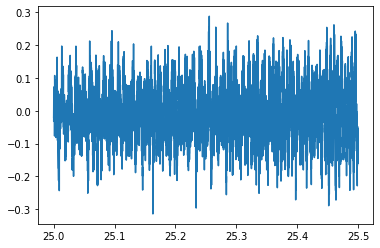
\includegraphics[width=0.75\textwidth]{lab1_fig2_2.png}
        \caption{Исходный звук}
        \label{fig:lab1_fig2_2}
\end{figure}

\section{Спектр звука}

Теперь рассмотрим спектр нашего полусекундного сегмента звука.

\begin{lstlisting}[caption=Спектр сегмента звука]
spectrum = segment.make_spectrum()
spectrum.plot(high=3000)
\end{lstlisting}

\begin{figure}[H]
        \centering
        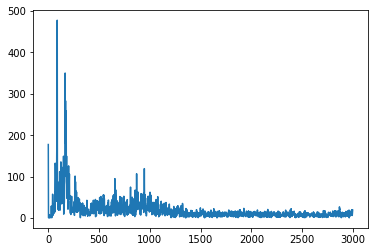
\includegraphics[width=0.75\textwidth]{lab1_fig2_3.png}
        \caption{Спектр сегмента звука}
        \label{fig:lab1_fig2_3}
\end{figure}

Теперь давайте рассмотрим основные и доминирующие частоты.

\begin{lstlisting}[caption=Основные и доминирующие частоты]
spectrum = segment.make_spectrum()
spectrum.plot(high=1000)
\end{lstlisting}

\begin{figure}[H]
        \centering
        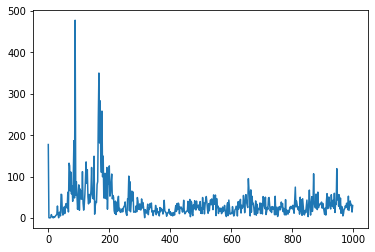
\includegraphics[width=0.75\textwidth]{lab1_fig2_4.png}
        \caption{Основные и доминирующие частоты}
        \label{fig:lab1_fig2_4}
\end{figure}

При помощи метода \texttt{spectrum.peaks()[:30]} определим доминирующий пик, который находится находится на частоте 88 Гц.

\begin{lstlisting}[caption=Отфильтрованный массив пиков]
[(477.12651815782436, 88.0),
 (349.78356868530363, 166.0),
 (282.7682770271516, 170.0),
 (257.9959018541909, 176.0),
 (241.34058048533615, 164.0),
 (186.61794990338055, 84.0),
 (181.12766751136527, 168.0),
 (177.34814169151826, 0.0),
 (157.95871927000582, 172.0),
 (149.43185101975794, 180.0),
 (149.14523507428788, 150.0),
 (135.43157096550385, 124.0),
 (132.31096277693203, 68.0),
 (126.03280864487395, 70.0),
 (125.78404373338199, 200.0),
 (122.03771045731844, 192.0),
 (121.9978844128709, 142.0),
 (119.22228552637446, 946.0),
 (116.56985643634354, 128.0),
 (111.97150490905403, 112.0),
 (110.96738906342934, 74.0),
 (110.30567932667302, 174.0),
 (107.97413765938968, 186.0),
 (106.82983478456184, 870.0),
 (106.16611169214379, 208.0),
 (101.22634883171585, 264.0),
 (100.31004880713746, 82.0),
 (99.62009343933141, 178.0),
 (99.24076695835758, 122.0),
 (95.08575904720958, 656.0)]
\end{lstlisting}

\section{Фильтрация звука}

Применим фильтр нижних частот.

\begin{lstlisting}[caption=Фильтрация и воспроизведение звука]
spectrum.low_pass(2000)
spectrum.make_wave().make_audio()
\end{lstlisting}

\begin{lstlisting}[caption=Визуализация фильтрации]
spectrum.make_wave().plot()
\end{lstlisting}

\begin{figure}[H]
        \centering
        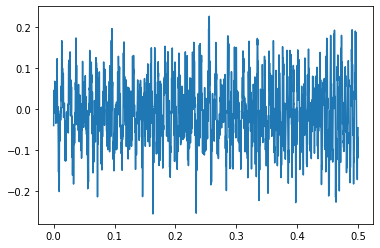
\includegraphics[width=0.75\textwidth]{lab1_fig2_5.png}
        \caption{Спектр сегмента звука}
        \label{fig:lab1_fig2_5}
\end{figure}

Как видно из графика, сигнал после фильтрации значительно поредел, а звук стал похож на воспроизведение его под водой или за стеной.

\chapter{Упражнение 1.3}
\section{Создание сложного сигнала}

Создадим сложный сигнал из объектов \texttt{SinSignal} и \texttt{CosSignal}.

\begin{lstlisting}[caption=Создание сложного сигнала]
signal = (thinkdsp.SinSignal(freq=140, amp=0.7) +
          thinkdsp.SinSignal(freq=440, amp=0.2) +
          thinkdsp.CosSignal(freq=640, amp=0.8))
signal.plot()
\end{lstlisting}

\begin{figure}[H]
        \centering
        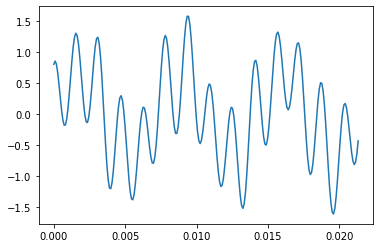
\includegraphics[width=0.75\textwidth]{lab1_fig3_1.png}
        \caption{Спектр сегмента звука}
        \label{fig:lab1_fig3_1}
\end{figure}

Достаточно интересный звук у нас получился, теперь попробуем его прослушать.

\begin{lstlisting}[caption=Воспроизведение сложного сигнала]
wave2 = signal.make_wave(duration=1)
wave2.apodize()
wave2.make_audio()
\end{lstlisting}

Полученный звук схож с чем-то инопланетным, будто я попал в какую-то вселенную Звёздных Войн. Выведем спектр полученного звука.

\begin{lstlisting}[caption=Визуализация сложного сигнала]
spectrum = wave2.make_spectrum()
spectrum.plot(high=2000)
\end{lstlisting}

\begin{figure}[H]
        \centering
        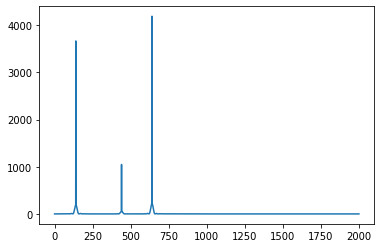
\includegraphics[width=0.75\textwidth]{lab1_fig3_2.png}
        \caption{Визуализация сегмента звука}
        \label{fig:lab1_fig3_2}
\end{figure}

\section{Добавление новой частоты}

Попробуем добавить новую частоту в наш имеющийся сигнал и прослушать полученный звук.

\begin{lstlisting}[caption=Добавление новой частоты и воспроизведение]
signal += thinkdsp.SinSignal(freq=1000)
signal.make_wave().make_audio()
\end{lstlisting}

Теперь слышно добавленную новую частоту, при чём более высокую, потому что \texttt{freq=1000}. Теперь звук более похож на набор цифр при звонке через стационарный телефон.

\chapter{Упражнение 1.4}

Для выполнения данного упражнения возьмём скачанный звук из \texttt{Упражнения 1.2}.

\begin{lstlisting}[caption=Загрузка и прослушивание звука]
wave3 = thinkdsp.read_wave('sounds/414062__felix-blume__machine-gears.wav')
wave3.normalize()
wave3.make_audio()
\end{lstlisting}

Теперь сделаем функцию \texttt{stretch}.

\begin{lstlisting}[caption=Функция stretch]
def stretch(wave, factor):
    wave.ts *= factor
    wave.framerate /= factor
\end{lstlisting}

Попробуем прослушать полученный звук, введя 0.25. По логике он должен ускориться в 4 раза.

\begin{lstlisting}[caption=Прослушивание ускоренного звука]
stretch(wave3, 0.25)
wave3.make_audio()
\end{lstlisting}

Теперь этот звук напоминает работающий блендер или мясорубку, что аж есть захотелось. Проверим работоспособность нашей функции визуализируя полученный звук.

\begin{lstlisting}[caption=Визуализация ускоренного звука]
wave3.plot()
\end{lstlisting}

\begin{figure}[H]
        \centering
        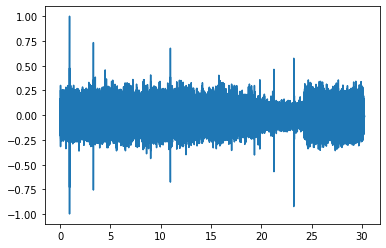
\includegraphics[width=0.75\textwidth]{lab1_fig4_1.png}
        \caption{Визуализация ускоренного звука}
        \label{fig:lab1_fig4_1}
\end{figure}

\chapter{Выводы}

Во время выполнения лабораторной работы получены навыки работаты со звуками, волнами и спектрами. Также я научился находить более высокие и фундаментальные пики, определять частоту, а также ускорять и замедлять звуки и строить графики.

\end{document}